
\section{SVD in R}

If \Mtx{A} is an $n \times p$ matrix, and the singular value decomposition of \Mtx{A} is given by $\Mtx{A} = \Mtx{U} \Mtx{S} \Mtx{V}^T$, the columns of the  matrix $\Mtx{V}^T$ are the eigenvectors of the square matrix $\Mtx{A}^T \Mtx{A}$ (sometimes refered to  as the minor product of \Mtx{A}). The singular values of \Mtx{A} are equal to the square roots of the eigenvalues of $\Mtx{A}^T \Mtx{A}$. 

The \verb|svd()| function computes the singular value decomposition of an arbitrary rectangular matrix. Below I demonstrate the use of the \verb|svd()| function and confirm the relationships described above:

\begin{R}
> A <- matrix(c(2,1,2,3),nrow=2)
> A
     [,1] [,2]
[1,]    2    2
[2,]    1    3
> a.svd <- svd(A)
> a.svd$u
           [,1]       [,2]
[1,] -0.6618026 -0.7496782
[2,] -0.7496782  0.6618026
# R uses the notation A = u d v' rather than A = u s v' 
> a.svd$d  
[1] 4.1306486 0.9683709
> all.equal(A, a.svd$u %*% diag(a.svd$d) %*% t(a.svd$v)) 
[1] TRUE
> AtA <- t(A) %*% A
> eigen.AtA <- eigen(AtA)
> eigen.AtA
$values
[1] 17.0622577  0.9377423
$vectors
          [,1]       [,2]
[1,] 0.5019268 -0.8649101
[2,] 0.8649101  0.5019268
> all.equal(a.svd$d, sqrt(eigen.AtA$values))
[1] TRUE
\end{R}

As we discussed in lecture, the eigenvectors of square matrix, \Mtx{A}, point in the directions that are unchanged by the transformation specified by \Mtx{A}.

\subsection{Writing our own PCA function}

In lecture we discussed the relationship between SVD and PCA.  Let's walk through some code that carries out PCA via SVD, and then we'll impliment our own PCA function.
%
\begin{R}
> i.sub <- subset(iris, select=-Species)
> i.ctr <- scale(i.sub, center=T, scale=F)
> i.svd <- svd(i.ctr)

> U <- i.svd$u
> S <- diag(i.svd$d)
> V <- i.svd$v

> pc.scores <- U %*% S
# compare to fig 5.5 in your workbook
> plot(pc.scores, asp=1, col=c('red', 'darkolivegreen', 'blue')[iris$Species], pch=16)

> n <- nrow(i.ctr)
> pc.sdev <- sqrt((S**2/(n-1)))
> pc.sdev
         [,1]      [,2]      [,3]      [,4]
[1,] 2.056269 0.0000000 0.0000000 0.0000000
[2,] 0.000000 0.4926162 0.0000000 0.0000000
[3,] 0.000000 0.0000000 0.2796596 0.0000000
[4,] 0.000000 0.0000000 0.0000000 0.1543862


> V
            [,1]        [,2]        [,3]       [,4]
[1,]  0.36138659 -0.65658877  0.58202985  0.3154872
[2,] -0.08452251 -0.73016143 -0.59791083 -0.3197231
[3,]  0.85667061  0.17337266 -0.07623608 -0.4798390
[4,]  0.35828920  0.07548102 -0.54583143  0.7536574
\end{R}
%
For comparison, here's what the builtin |prcomp| function gives us:
\begin{R}
> i.pca <- prcomp(i.ctr)
> i.pca$sdev
[1] 2.0562689 0.4926162 0.2796596 0.1543862
> i.pca$rotation
                     PC1         PC2         PC3        PC4
Sepal.Length  0.36138659 -0.65658877  0.58202985  0.3154872
Sepal.Width  -0.08452251 -0.73016143 -0.59791083 -0.3197231
Petal.Length  0.85667061  0.17337266 -0.07623608 -0.4798390
Petal.Width   0.35828920  0.07548102 -0.54583143  0.7536574
\end{R}

Now that we have a sense of the key calculations, let's turn this into a function. Save the following code in file named |mypca.R|.

\bigskip
\begin{codeblock}
# a user defined version of principal components analysis
PCA <- function(X, center=T, scale=F){
   x <- scale(X, center=center, scale=scale)
   n <- nrow(x)
   p <- ncol(x)
   
   x.svd <- svd(x)
   U <- x.svd$u
   S <- diag(x.svd$d)
   V <- x.svd$v
   
   # check for zero eigenvalues
   zeros <- rep(0, p)
   tolerance = .Machine$double.eps^0.5
   has.zero.singval <- any(x.svd$d <= tolerance)
   if(has.zero.singval)
     print("WARNING: Zero singular values detected")
  
   pc.scores <- U %*% S
   pc.sdev <- diag(sqrt((S**2/(n-1))))
   return(list(vectors = V, scores=pc.scores, sdev = pc.sdev))
}
\end{codeblock}

Note I also included some code to warn the user when the covariance matrix is singular. Use the help to read about variables defined in `.Machine`.

Let's put our function through it's paces:
%
\begin{R}
> source('mypca.R')
> iris.pca <- PCA(i.sub)
> plot(iris.pca$scores, asp=1)

> sing.pca <- PCA(t(i.sub))  # should have singular values equal to zero
[1] "WARNING: Zero singular values detected"

> tree.pca <- PCA(trees)
> tree.pca$sdev
[1] 17.1834214  4.9820035  0.7485858
> prcomp(trees)$sdev # compare to prcomp
[1] 17.1834214  4.9820035  0.7485858
\end{R}

To bring things full circle, let's make sure that the covariance matrix we reconstruct from our PCA analysis is equal to the covariance matrix calculated directly from the data set:
\begin{R}
> n <- nrow(i.sub)
> V <- iris.pca$vectors
> S <- diag( sqrt(iris.pca$sdev**2 * (n-1)) ) # turn sdev's back into singular values
> reconstructed.cov <- (1/(n-1)) * V %*% S %*% S %*% t(V) # see pg. 11 of slides
> all.equal(reconstructed.cov, cov(i.sub), check.attributes=F)
[1] TRUE  
\end{R}
Great! I seems like things are working as expected.

\section{Creating Biplots in R}

To illustrate the construction of biplots we'll use the iris data set. The built-in R function is |biplot()|. 

\begin{R}
# leave out the Species variable
> iris.vars <- subset(iris, select=-Species) 
# read the prcomp docs and note differnces from princomp
> iris.pca <- prcomp(iris.vars)
> summary(iris.pca)

Importance of components:
                          PC1     PC2    PC3     PC4
Standard deviation     2.0563 0.49262 0.2797 0.15439
Proportion of Variance 0.9246 0.05307 0.0171 0.00521
Cumulative Proportion  0.9246 0.97769 0.9948 1.00000

> ?biplot  # read the help for biplot
> ?biplot.prcomp  # more detailed info on how biplot works with objects return by prcomp
> biplot(iris.pca, scale=1)  # scale = 1 - alpha
# change the biplot scaling - how does this differ?
> biplot(iris.pca, scale=0)  
\end{R}

Note that the |scale| argument to biplot sets the $\alpha$ value we discussed during lecture, however |scale| = $1-\alpha$ (i.e. if |scale| = 1, $\alpha=0$, and if |scale| = 0, $\alpha=1$).

\medskip
\begin{assignment}
\begin{enumerate}
  \item Apply PCA (on the covariances) to the \verb|yeast-subnetwork-clean.txt| data set.
  \item Create biplots in the first two principal components using both $\alpha=0$ and $\alpha=1$ (i.e. the |scale| argument to biplot). 
  \item In your biplots change the labels for the observations to integers using the \verb|xlabs| argument to \verb|biplot()|. To make the plot more readable use the |cex| argument to |biplot| to make the font size for the observations half the size of the variable labels.
  \item An obvious pattern emerges in the biplot with respect to the gene MEP2. What is this pattern? What subset of conditions (rownames) is most closely related to the vector representing MEP2?
\end{enumerate}     
\end{assignment}



% \subsection{`Seriating' samples using SVD}

% The term `seriation' refers to the process of finding an ordering of objects or variables such that they follow a natural ordering with respect to some criteria (e.g. time, similarity, etc.). One way to think about this problem is in terms of ordering objects on a line (i.e. a 1D approximation).  Since we've learned that SVD can be used to provide optimal approximations (in the least squares sense) it seems natural to apply the technique to the problem of seriation. We'll illustrate this application by seriating both experimental conditions (samples) and variables (genes) for the yeast expression data set we've been working with.  There's some support for the assertion that seriation by SVD is a better method for re-ordering data matrices for heat maps than the more commonly used hierarchical clustering methods that you see in many microarray papers (Wilkinson, L. and M. Friendly. The History of the Cluster Heat Map. The American Statistician. May 1, 2009, 63(2): 179-184. \href{http://dx.doi.org/10.1198/tas.2009.0033}{doi link}) 



% \begin{R}
% >>> from matplotlib import pyplot
% >>> import numpy as np, numpy.linalg as la
% >>> # first let's look at the original matrix
% >>> yeast = np.loadtxt('yeast-subnetwork-clean.txt',skiprows=1, usecols=range(1,15))
% >>> yeast.shape
% (173, 14)
% >>> fig = pyplot.figure(figsize=(4,8))
% >>> ax = pylab.imshow(yeast, cmap='seismic')
% >>> fig.axes[0].set_aspect(0.2)
% >>> fig.show() 
% \end{python}

% Since we're going to be creating several figures you essentially the same code let's take a moment to create a function that will take care of the key steps for us.

% \begin{codeblock}[python]
% # yeastdraw.py
% from matplotlib import pylab, pyplot

% def draw_yeast_matrices(matrices = [], titles = [], cmap='seismic'):
%     """ draw an image represent of a set of matrices
    
%     matrices and titles should be lists containing np.arrays and strings
%     respectively. See the matplotlib docs for color maps other than 'seismic'
%     """
%     nmtx = len(matrices)
%     width = nmtx * 4
%     height = 8
    
%     fig = pyplot.figure(figsize=(width,height))
    
%     # look at the Python docs to read about how the enumerate fxn
%     for i, mtx in enumerate(matrices):
%         fig.add_subplot(1, nmtx, i+1)
%         ax = pylab.imshow(mtx, cmap=cmap)
%         fig.axes[i].set_aspect(0.2)
%         try:  # try and set title
%             fig.axes[i].set_title(titles[i])
%         except IndexError:  # if the title doesn't exist
%             pass            # just continue with the plotting tasks
%     return fig
    
% \end{codeblock}

% Having created that function we can now put it to use to visualization our seriation of the yeast expression data set.


% \begin{python}
% >>> import yeastdraw as yd    
% >>> # now do the SVD   
% >>> u,s,vt = la.svd(yeast)
% >>> u1 = u[:,0] # first column of u

% # ths specifies how to sort the samples relative to the largest left 
% # singular vector
% >>> u1sort = np.argsort(u1) 
% # lookup the help for argsort so you understand what it does
% >>> help(np.argsort)  
% >>> s1 = yeast[u1sort] # yeast data with rows sorted by u1

% # now create a figure showing original and new ordering
% >>> fig = yd.draw_yeast_matrices([yeast, s1],
%             ['Original ordering', 'SVD re-ordering of rows'])
% >>> fig.show()

% # let's repeat it where we sort both rows and cols
% >>> v1sort = np.argsort(vt[0])
% >>> s2 = s1[:,v1sort]
% >>> fig = yd.draw_yeast_matrices([yeast,s1, s2],
%         ['Original ordering', 'SVD re-ordering of rows',
%         'SVD, rows and cols re-ordered'])
% >>> fig.show()
% \end{python}

\section{Data compression and noise filtering using SVD}

Two common uses for singular value decomposition are for data compression and noise filtering. Will illustrate these with two examples involving matrices which represent image data. This example is drawn from an article by David Austin, found on a tutorial about SVD at the American Mathematical Society Website (\href{http://www.ams.org/samplings/feature-column/fcarc-svd}{link}).

\subsection{Data compression}

Download the file |zeros.dat| from the course wiki. This is a $25 \times 15$ binary matrix that represents pixel values in a simple binary (black-and-white) image.

\begin{R}
> z <- read.delim('zero.dat',header=F)
> z
   V1 V2 V3 V4 V5 V6 V7 V8 V9 V10 V11 V12 V13 V14 V15
1   1  1  1  1  1  1  1  1  1   1   1   1   1   1   1
2   1  1  1  1  1  1  1  1  1   1   1   1   1   1   1
... output truncated ...

# we'll use the image() function to visualize z
> image(1:15,1:25,t(z),col=c('black','white'),asp=1)    
\end{R}

This matrix data is shown below in a slightly different form that emphasizes the individual elements of the matrix.  As you can see, this matrix can be thought of as being composed of just three types of vectors.


\begin{figure}[ht!]
\begin{center}
\subcaptionbox{The `zero' matrix.}[0.4\linewidth]{%
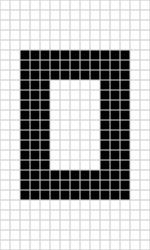
\includegraphics[height=1in]{./figures/hands-on6/zero.jpg}% 
}
\subcaptionbox{The three vector types in the `zero' matrix.}[0.4\linewidth]{%
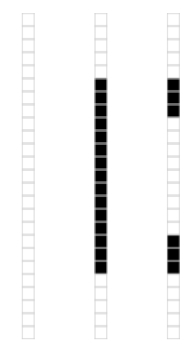
\includegraphics[height=1in]{./figures/hands-on6/zero-vecs.jpg}% 
}
\end{center}
\end{figure}

If SVD is working like expected it should capture that feature of our input matrix, and we should be able to represent the entire image using just three singular values and their associated left- and right-singular vectors.

\begin{R}
> zsvd <- svd(z)
> round(zsvd$d,2)
 [1] 14.72  5.22  3.31  0.00  0.00  0.00  0.00  0.00  0.00  0.00  0.00  0.00  0.00  0.00
[15]  0.00
> D <- diag(zsvd$d[1:3])
> D
         [,1]     [,2]     [,3]
[1,] 14.72425 0.000000 0.000000
[2,]  0.00000 5.216623 0.000000
[3,]  0.00000 0.000000 3.314094
> U <- zsvd$u[,1:3]
> V <- zsvd$v[,1:3]
> newZ <- U %*% D %*% t(V)
> all.equal(newZ, zmatx, check.attributes=F)
[1] TRUE

# and let's double check using the image() function
> image(1:15,1:25,t(newZ),col=c('black','white'),asp=1)
\end{R}

Our original matrix required $25 \times 15$ ($= 375$) storage elements. Using the SVD we can represent the same data using only $15 \times 3 + 25 \times 3 + 3 = 123$ units of storage (corresponding to the truncated U, V, and D in the example above). Thus our SVD allows us to represent the same data with at less than $1/3$ the size of the original matrix. In this case, because all the singular values after the 3rd were zero this is a lossless data compression procedure. 


\subsection{Noise filtering using SVD}

The file |noisy-zero.dat| is the same 'zero' image, but now sprinkled with Gaussian noise draw from a normal distribution ($N(0,0.1)$. As in the data compression case we can use SVD to approximate the input matrix with a lower-dimensional approximation. Here the SVD is `lossy' as our approximation throws away information.  In this case we hope to choose the approximating dimension such that the information we lose corresponds to the noise which is `polluting' our data. 

\begin{R}
> nz <- as.matrix(read.delim('noisy-zero.dat',header=F))
> dim(nz)
[1] 25 15
> x <- 1:15
> y <- 1:25
# create a gray-scale representation of the matrix
> image(x,y,t(nz),asp=1,xlim=c(1,15),ylim=c(1,25),col=gray(seq(0,1,0.05)))
> round(nz.svd$d,2)
 [1] 13.63  4.87  3.07  0.40  0.36  0.31  0.27  0.26  0.21  0.19  0.13  0.11  0.09  0.06
[15]  0.04
# as before the first three singular values dominate
> nD <- diag(nz.svd$d[1:3])
> nU <- nz.svd$u[,1:3]
> nV <- nz.svd$v[,1:3]
> approx.nz <- nU %*% D %*% t(nV)    

# now plot the original and approximating matrix side-by-side
> par(mfrow=c(1,2))
> image(x,y,t(nz),asp=1,xlim=c(1,15),ylim=c(1,25),col=gray(seq(0,1,0.05)))
> image(x,y,t(approx.nz),asp=1,xlim=c(1,15),ylim=c(1,25),col=gray(seq(0,1,0.05)))
\end{R}

As you can see from the images you created the approximation based on the approximation based on the SVD manages to capture the major features of the matrix and filters out much of (but not all) the noise.

\section{Image Approximation Using SVD in R}

R doesn't have native support for common image files like JPEG and PNG.  However, there are a couple of packages we call install that will allow us to read in such files and treat them as matrices:
%
\begin{R}
> install.packages("png", dependencies=T)
> install.packages("jpeg", dependencies=T)
\end{R}

The |png| and |jpeg| libraries provide simple functions for reading and writing image files.  The following code shows how to read in the |chesterbw.jpg| image which can be found in the course datasets. An alternative package is |ReadImages| which provides more functions for manipulating image data, including a funciton to convert color images to greyscale.

The function |grid.raster| in the |grid| library can be used to draw the matrix of image data returned from the |readJPEG|.  There is also a lower-level |rasterImage()| function that can be used to draw images, as shown below.
%
\begin{R}
> library(jpeg)
> img <- readJPEG("chesterbw.jpg")
> dim(img)
[1] 556 605
> typeof(img)
[1] "double"
> class(img)
[1] "matrix"
> ny <- dim(img)[1]  # rasterImage will draw rows along vertical axis
> nx <- dim(img)[2]
> max.pixels <- max(nx,ny)
> plot(0:max.pixels, 0:max.pixels, type='n', xlab='', ylab='',asp=1)
> ?rasterImage
> rasterImage(img, 0, 0, nx, ny)
> library(grid)
> ?grid.raster
> grid.raster(img)  # more convenient but less flexible than rasterImage
\end{R}
The output of the code above is shown in Fig~\ref{fig:chester}.
\begin{figure}[ht!]
  \center{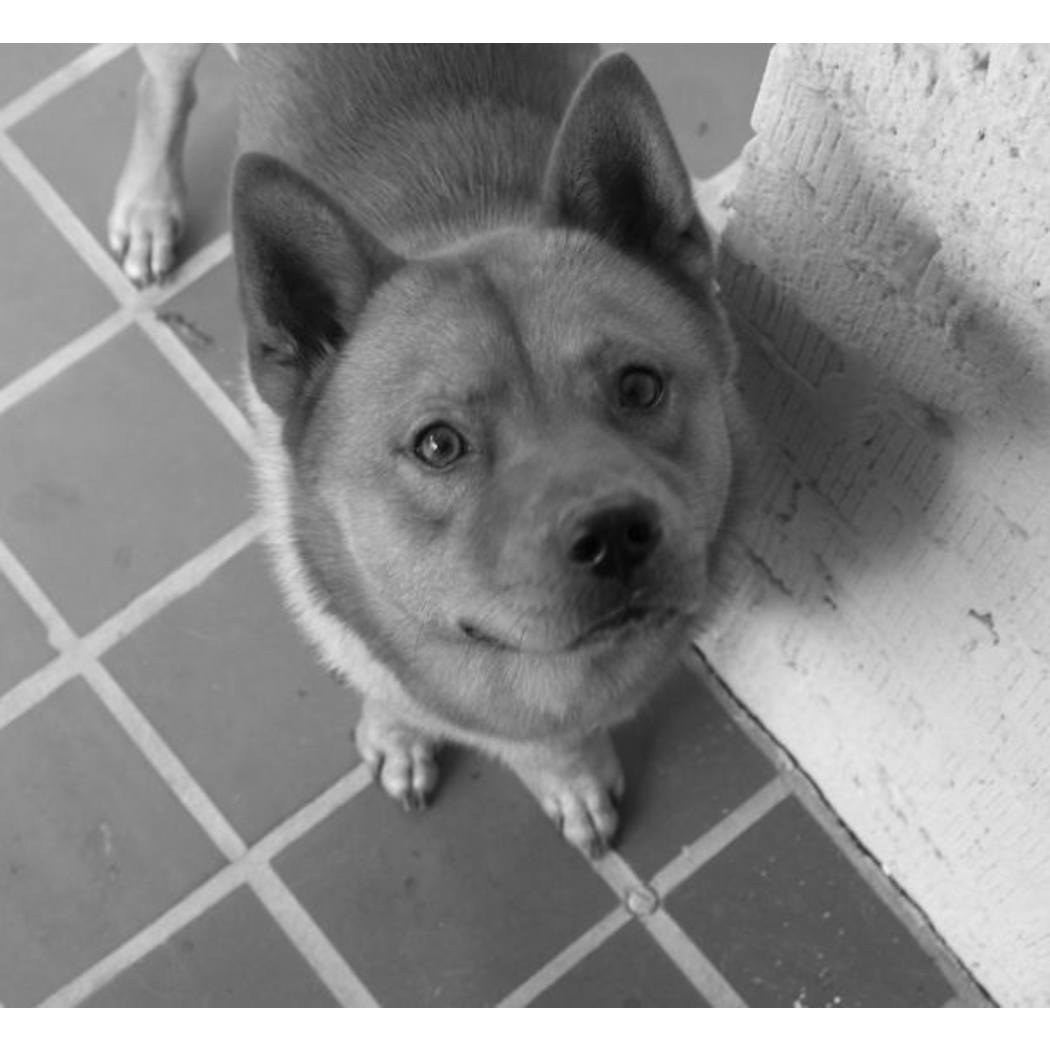
\includegraphics[width=0.33\textwidth]{./figures/hands-on6/fig-chesterorig.pdf}}
  \caption{My ever-faithful companion Chester.\label{fig:chester}}
\end{figure}


Now we'll use SVD to create a low-dimensional approximation of this image.
%
\begin{R}
> img.svd <- svd(img)
> U <- img.svd$u
> S <- diag(img.svd$d)
> Vt <- t(img.svd$v)

> U15 <- U[,1:15]  # first 15 left singular vectors
> S15 <- S[1:15,1:15]  # first 15 singular values
> Vt15 <- Vt[1:15,]  # first 15 right singular values, NOTE: we're getting rows rather than columns here

> approx15 <- U15 %*% S15 %*% Vt15
> grid.raster(approx15)
\end{R}
%
The output of our approximate image is shown in Fig~\ref{fig:chester15}.
\begin{figure}[ht!]
  \center{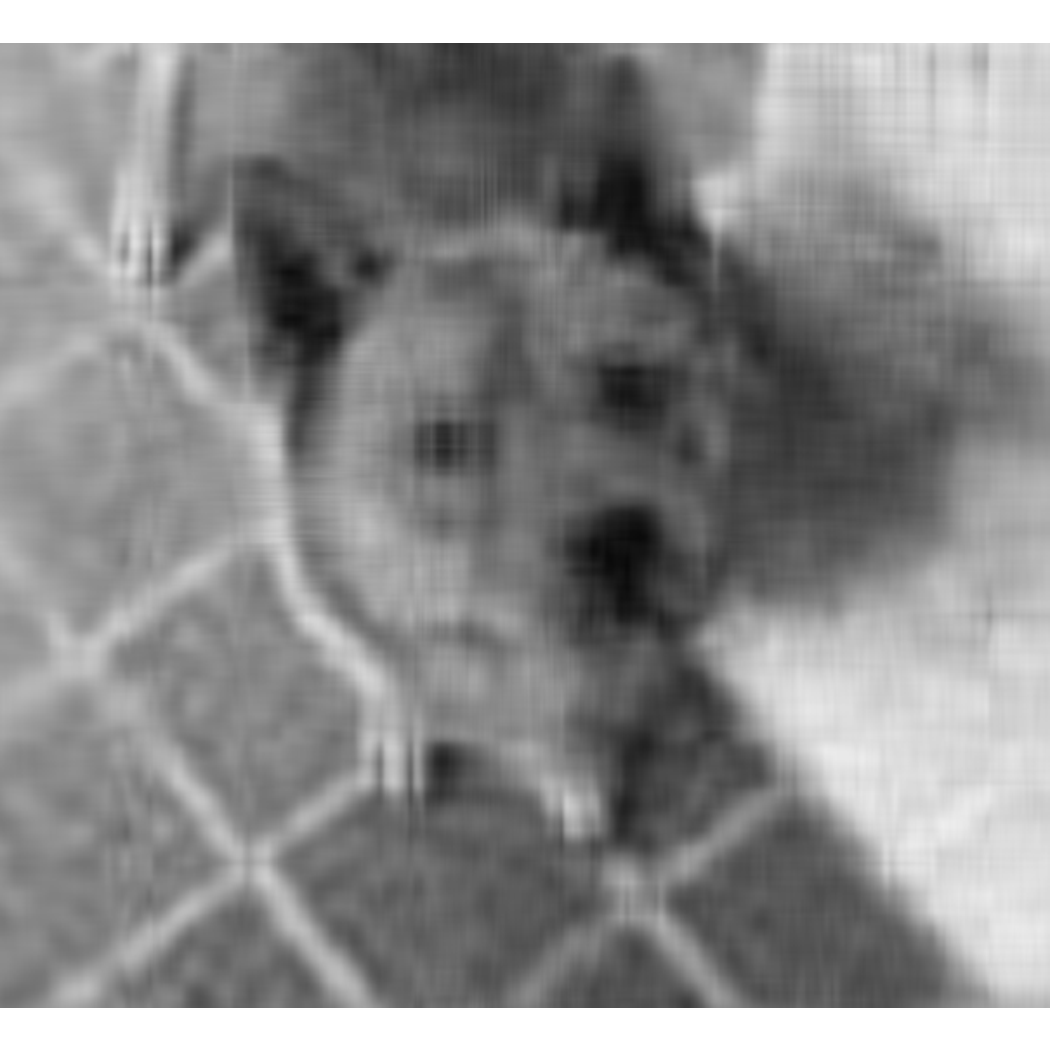
\includegraphics[width=0.33\textwidth]{./figures/hands-on6/fig-chesterapprox15.pdf}}
  \caption{A low-dimensional approximation of Chester.\label{fig:chester15}}
\end{figure}


Above we created a rank 15 approximation to the rank 556 original image matrix. This approximation is crude (as judged by the visual quality of the approximating image) but it does represent a very large savings in space. Our original image required the storage of $605 \times 556 = 336380$ integer values. Our approximation requires the storage of only $15 \times 556 + 15 \times 605 + 15 = 17430$ integers. This is a saving of roughly 95\%. Of course, as with any lossy compression algorithm, you need to decide what is the appropriate tradeoff between compression and data loss for your given application.


\begin{assignment}
% \small

Write a function, |svd_img()|, that automates the creation of a lower dimensional approximation of a grayscale image using SVD.  

\begin{enumerate}
  \item Your function should take as input a matrix representing the original image and an integer specifying the approximating dimension -- i.e. function will be called as \verb|svd_img(imgmtx,dim)|.  

  \item Your function should return a list of two objects: 1) an array representing the approximated image; and 2) an array representing the difference between the original and approximating images.

  \item Test your function on various images using a variety of approximating dimensions (e.g. 5,10, 25, 50, 100, 250) on the \verb|chesterbw.jpg| image.
\end{enumerate}


In addition to your code consider the following questions:

\begin{itemize}
\item When analyzing \texttt{chesterbw.jpg}, at some approximating dimensions you'll notice interesting artifacts. How do these relate to the original image? 

\item What is the lowest approximating dimension where you would you consider the image to be recognizable as a dog?
 
\item At what approximating dimension would you judge the  image to be ``close enough"  to the original by the casual observer? What is the storage saving of this approximation relative to the original image?

%\item How does the difference array (original - approximating) change as the approximating dimension changes? Is there a particular type of image information that seems most prominent in the difference array?
\end{itemize}


\end{assignment}




